\documentclass[12pt]{article}

\usepackage{sbc-template}

\usepackage{graphicx,url}
\usepackage[algoruled,longend]{algorithm2e}
\usepackage[brazil]{babel}   
\usepackage[utf8]{inputenc}  
\usepackage{enumitem}
\setdescription{leftmargin=\parindent,labelindent=\parindent}
     
\sloppy

\title{Algoritmo Genéticos Paralelo: uma abordagem hierárquica}

\author{Derik Evangelista Rodrigues da Silva\inst{1}, Raphael Henrique Ferreira de Andrade\inst{1}, \\Eduardo Spinosa\inst{1}}

\address{Departamento de Informática -- Universidade Federal do Paraná
  (UFPR)\\
  Caixa Postal 19081 -- 81531-980 -- Curitiba -- PR -- Brasil
  \email{\{dersilva, rhfandrade, spinosa\}@inf.ufpr.br}
}

\begin{document} 

\maketitle

\begin{abstract}
  @TODO Abstract
\end{abstract}
     
\begin{resumo} 
  @TODO Resumo
\end{resumo}


\section{Introdução}

% O Algoritmo Genético (GA), frequentemente referenciado como \emph{algoritmos genéticos}, foi desenvolvido por John Holland na Universidade de Michigan, nos anos 70 (\cite{luke2009}).

Algoritmo Genetico (\emph{Genetic Algorithm} -- GA) são algoritmos de busca inspirados no processo de evolução e seleção natural \cite{goldberg1989} e tem tido grande sucesso em problemas de busca e de otimização, principalmente quando o espaços de busca é grande, complexo ou pouco conhecido, onde métodos de buscas convencionais (enumerativos, heurísticos, ...) não são apropriados \cite{herrera1998}. 

Um GA sequencial inicia-se gerando um conjunto de indivíduos para formar uma população inicial. Cada indivíduo representa uma possível solução do problema. Usando uma função de avaliação (chamada de função \emph{fitness}), mede-se a qualidade de cada indivíduo desta população. O cálculo do \emph{fitness} é, geralmente, o processo mais custoso de um GA \cite{paraleltax}. Seleciona-se aleatoriamente, então, um subconjunto de indivíduos desta população e neste é aplicado operadores estocásticos de seleção, mutação e cruzamento. Por fim, os indivíduos menos adaptados (ou seja, com pior \emph{fitness}) são descartados, para dar lugar a indivíduos mais bem adaptados.

% @TODO Colocar exemplos de sucesso!
Apesar do sucesso em muitas aplicações em diferentes domínios, existem, de acordo com \cite{paraleltax}, algums problemas que podem ser resolvidos com o uso de um Algoritmo Genético Paralelo (\emph{Parallel GA} -- PGA):

\begin{itemize}
  \item Para alguns tipos de problemas, o tamanho da população precisa ser muito grande, requerendo, consequentemente, uma grande quantidade de memória, podendo impossibilitar a execução eficiente em uma única máquina.
  \item O cálculo do \emph{fitness} consome muito tempo. Há registros na literatura de uma única execução consumindo mais de 1 ano de CPU.
  \item GA's sequencias podem ficar presos em regiões sub-ótimas, ficando impossibilitados de encontrar uma melhor solução. PGA's podem buscar em multiplos subespaços de busca em paralelo, e tem menos chance de ficar preso em regiões sub-ótimas.
\end{itemize}

O motivo mais importante para se estudar PGAs, ainda segundo \cite{paraleltax}, é que em muitos casos eles tem uma melhor performance do que os sequenciais, mesmo quando o paralelismo é simulado em uma máquina convencional. 

Este trabalho tem como objetivo comparar três tipos de arquiteturas de PGAs: múltiplas populações, arquitetura mestre-escravo e um híbrido de ambas, ou seja, uma combinação de múltiplas populaçõoes com mestre-escravo, aplicadas a otimização de funções. Além disso, compararemos os resultados com um GA sequencial convencional.

\section{Revisão de literatura} % (fold)
\label{sec:revisao_bibliogragica}

%Algoritmo Genetico: Origem, funcionamento, usos comuns
%AG Paralelo: concepcao, hierarquias, 

O Algoritmo Genético foi desenvolvido por John Holland na Universidade de Michigan, em 1970 \cite{holland1975}, inspirado no processo de seleção natural e evolução, e apresenta uma alternativa as técnicas clássicas de otimização, usando buscas aleatórias dirigidas para localizar soluções ótimas em espaços de buscas complexos \cite{gasurvey}. O objetivo original de Holland não era construir um algoritmo que resolvesse um problema específico, mas formalizar o estudo do fenômeno de adaptação da mesma forma que este acontece na natureza e desenvolver mecanismos de importar este comportamento em sistemas computacionais \cite{geintro1998}.

Tendo sua inspiração na biologia, alguns termos desta área são usados para descrever o GA \cite{luke2009}:
\begin{description}
	\item [Indivíduo] Solução candidata;
	\item [População] Conjunto de indivíduos;
	\item [Filhos e Pais] Um filho é uma cópia perturbada de seu pai (ambos são indivíduos);
	\item [\emph{Fitness} (Adaptabilidade)] Medida de qualidade de dada solução; 
	\item [Função de \emph{Fitness}] Função de qualidade. 
  \item [Seleção] Escolha de indivíduos, baseado em seu \emph{fitness};
  \item [Mutação] Pequena perturbação na solução;
  \item [Recombinação / Cruzamento] Grande perturbação na estrutura do indivíduo. Geralmente gera dois filhos recombinando a estrutura de seus pais.
  \item [Genoma / Genótipo] Estrutura do indivíduo;
  \item [Geração] População gerada em cada ciclo do algoritmo, que envolve as funções e transformações previamente definidas.
 \end{description}

O algoritmo apresentado em \cite{holland1975} é usualmente chamado de canônico \cite{yang2002} ou Algoritmo Genético Simples (SGA) \cite{gasurvey} e trabalha, essencialmente, com indivíduos sendo um vetor de bits, ou seja, a solução é codificada em termos de 0 e 1. Como método de seleção, o SGA usa o esquema de \emph{roleta}, onde um determinado indivíduo tem mais chance de ser escolhido para procriar dependendo de seu \emph{fitness}
 calculado.

Algumas variações foram apresentadas, como a inclusão de elitismo \cite{dejong1975}, que consiste em manter um número de indivíduos com melhor \emph{fitness} de uma geração para outra, o \emph{Steady-State Genetic Algorithm}  \cite{whitley1988}, que atualiza a população assim que os filhos são gerados, descartando-os ou inserindo-os no lugar de alguns de indivíduos piores da população e o \emph{Tree-Style Genetic Programming Pipeline}, que utiliza uma forma diferente de procriação: com 90\% de probabilidade, dois pais serão selecionados e será efetuado o cruzamento convencional e, por outro lado, com 10\% de probabilidade, será selecionado apenas um pai, que será copiado para a nova população. Existem versões, também, que se preocupam em adaptar as taxas de cruzamento e mutação em tempo de execução e abordagens híbridas, como efetuar uma busca local em cada indivíduo, usando outro algoritmo \cite{bersing1994} \cite{katare2000}.

Muitos dos algoritmos evolutivos são inerentemente paralelos \cite{hoverstad2010}, pela natureza independente de suas operações \cite{albasurvey}, e o paralelismo surge como uma alternativa para melhorar a eficiência dos GAs. 

Os algoritmos genéticos paralelos (PGA) não são apenas versões paralelas de GA sequenciais. De fato, na maioria dos casos, o todo (PGA) tem melhor performance que a soma das sub-partes que o compões \cite{albasurvey}.

A maneira com que os GAs são paralelizados depende dos seguintes elementos \cite{paraleltax}: 
\begin{itemize}
  \item Como é calculado a função \emph{fitness} e como a mutação é aplicada;
  \item Se multiplas subpopulações \emph{demes} são usadas;
  \item Se multiplas populações são usadas e como os indivíduos interagem e;
  \item Como a seleção é aplicada (globalmente ou localmente);
\end{itemize}
% @TODO REVISÃO AG PARALELO: HIERARQUIAS

Dos parâmetros acima, pode-se extrair quatro tipos principais de PGA \cite{cantu1998}: 
\begin{itemize}
  \item Mestre-escravo \emph{(Master Slave)}: globais de uma única população;
  \item Única população com paralelização \emph{fine-grained};
  \item Múltiplas populações com paralelização \emph{coarsed-grained} e;
  \item Combinação dos métodos acima
\end{itemize}
Onde \emph{fine-grained} refere-se a algoritmos paralelos com frequente comunicação entre as partes, enquanto \emph{coarse-grained} refere-se ao contrário.

No esquema mestre-escravo, usa-se uma única população e paraleliza-se os cálculos de \emph{fitness} nos processodores. Os \emph{fine-grained} PGA (FGPGA) são usados em máquinas massivamente paralelas e consistem de uma única população espacialmente estruturada e os \emph{coarsed-grained} PGA (CGPGA, também chamados de GA Distribuídos) consistem de múltiplas populações (também chamado de \emph{demes} ou \emph{ilhas}) que evoluem em paralelo e trocam indivíduos ocasionalmente (esta troca é chamada de \emph{migração}). Aos esquemas que combinam multiplas populações com mestre-escravo ou FGPGA dá se o nome de \emph{hierárquicos} (HPGA).

O primeiro PGA foi proposto em 1987 por Pettey, Leuze e Grefenstette e utilizava o esquema de multiplas populações, migrando sempre o melhor \cite{albasurvey}. \cite{tanese1989} utilizou o esquema de populações distribuídas e obteve bons resultados com migração de 20\% da população a cada 20 gerações. \cite{asparagos1989} usavam um FGPGA e aplicava \emph{hill climbing} caso não obtivesse nenhuma melhora em um determinado número de gerações. \cite{adamidis1996} utilizam múltiplas ilhas e é particularmente interessante pois cada uma das ilhas possuem suas próprias probabilidades de mutação, cruzamento e operadores especializados. \cite{wilson2010} apresentam um PGA que faz uso dos diversos núcleos das placas de vídeo de consoles de video-game, obtendo bons resultados em tempo de execução reduzido.

\cite{lim2007} apresentam um arcabouço para desenvolvimento de HPGA com suporte à computação em grade, e sugeriram, através de um estudo empírico utilizando problemas de \emph{benchmark} e problemas reais, que pode-se obter uma aceleração desde que os limites do custo da função \emph{fitness}, tamanho do \emph{cluster} e \emph{overheads} na comunicação sejam satisfeitos.

 \cite{zeng2007} sugere um novo PGA, chamado de \emph{asynchronous heterogeneos hierarchical parallel genetic algorithm} (AHHPGA) aplicado para a resolução do \emph{Redundancy Allocation Problem}, e usa um modelo \emph{coarsed-grained} como camada superior e um modelo \emph{fine-grained} na camada inferior. Este modelo proposto possui multiplas populações heterogêneas, com diferentes níveis de exploração das soluções e diferentes topologias em cada subpopulação. A migração acontece de forma assíncrona, tanto o envio quanto a recepção de novos indivíduos. Os resultados obtidos por este modelo foram ligeiramente melhores do que os obtidos por um GA tradicional, mas a faltou uma análise estatística elaborada para corroborar o modelo. 

\cite{heesung2009} apresentam um modelo hierarquico com competição justa, ou seja, a população é divida em camadas (ou classes) de acordo com o \emph{fitness} do indivíduo e estes só competem com outros da mesma camada. Indivíduos mudam de classe quando atingem um grau de aptidão superior ao limiar de aceitação da outra classe. Desta forma, mantém-se uma maior diversidade na população, comprovada pelos testes realizados.

 \cite{benitez2010} apresentam um modelo hierárquico (multiplas populações \emph{coarsed-grained} no nível mais alto e, no nível mais baixo, mestre-escravo) para o problema de desdobramento de proteínas, obtendo melhores resultados em 7 de 10 em comparação com o \emph{benchmark} de outro PGA não-hierárquico.


\section{Experimentos} % (fold)
\label{sec:experimentos}

\subsection{Problema} % (fold)
\label{sub:problema}

Três funções de \emph{benchmark} da literatura foram escolhidas, duas definidas em \cite{dejong1975} e a função de Rastrigin. Aplicamos estas funções ao problema de minimização. As definições das funções foram extraídas de \cite{luke2005}.

A primeira função de \cite{dejong1975}, a Função Esfera (\emph{Sphere Function}), é relativamente simples. Não possui ótimos locais e é facilmente resolvida por um GA. O valor de $x$ varia entre $-5.12$ e $+5.12$.

\begin{equation} \label{eq:spher}
  f(Sphere) = \sum_{i = 1}^{n} x_{i}^2
\end{equation}

A segunda função utilizada foi a Função \emph{Rotated Hyper-ellipsoid function} é continua, convexa e unimodal. O valor de $x$ varia entra $-5.12$ e $+5.12$.

\begin{equation} \label{eq:step}
  f(Step) = \sum_{i = 1}^{n}\sum_{j=1}^{i} x_j^2
\end{equation}

A função de Rastrigin é outro problema muito difícil já que define um espaço de busca muito grande, com $n = 20$ com valores entre $-5.12$ e $+5.12$. Além disso, possui muitos ótimos locais. Esta combinação faz com que muitos algoritmos possuam grande dificuldade para encontrar a solução ótima. As variáveis $A$ e $\omega$ controlam a frequencia e modulação do espaço de busca. No estudo feito, $A = 10$ e $\omega = 2\pi$;

\begin{equation} \label{eq:rast}
  f(Rastrigin) = 10 \times n + \sum_{i=1}^{n} \left[ x_{i}^2 - 10 \times cos(2 \pi x_i)\right]
\end{equation}


% \[
%   F2 = \sum_{i = 0}^{n-1} (100 \times (x_{i+1} - x_{i}^2)^2 + (x_i - 1)^2)
% \]

Os códigos foram desenvolvido em C, com uso da biblioteca \emph{OpenMP} para paralelização. Todos os testes foram executados em uma máquina Linux de 64bits com 4 \emph{cores} de processamento.

% subsubsection problema (end)

\subsection{Representação e Parâmetros} % (fold)
\label{sub:representacao}

Os casos de testes consistiam em achar um conjunto de elementos $(x_0, x_1, x_2, \dots x_n)$ que minimizasse as funções definidas na seção \ref{sub:problema}.

Utilizamos o método definido em \cite[p. 3]{gasurvey} para representar os números em ponto flutuante. Substituimos o valor do número pelo seu equivalente em inteiro, multiplicando por $10^p$, onde $p$ é o grau de precisão (casas decimais). Este número inteiro é então representado em uma \emph{string de bits}, em binário. Como as funções definidas em \ref{sub:problema} possuem domínio entre o intervalo $-5.12$ e $+5.12$, utilizamos uma \emph{string de bits $v$} de 10 posições, sendo a posição $v_0$ referente ao sinal, para cada número que queremos representar.

O cruzamento dá-se de forma convencional, pelo método \emph{One-point Crossover}: considere dois indivíduos $v$ e $q$ e $m$ o tamanho do indivíduo; os indivíduos $z$ e $w$, resultados do cruzamento de $v$ e $q$ serão:
\[
  z = [v_0, v_1, v_2, \dots, v_n, q_{n+1}, q_{n+2}, \dots q_m]
\]
\[
   w = [q_0, q_1, q_2, \dots, q_n, v_{n+1}, v_{n+2}, \dots v_m]
\]
Onde $n$ é um valor escolhido de forma aleatória, $ 0 \le n < m$.
A taxa de cruzamento é de 100\%.

A mutação também é realizada da forma clássica: seja $v$ um indivíduo. Para todo $x_i \in v$, com probabilidade $p$, faça $x_i = \overline{x_i}$, onde:
 \begin{displaymath}
   \overline{x_i} = \left\{
     \begin{array}{lr}
       0 & : x_i = 1 \\
       1 & : x_i = 0
     \end{array}
   \right.
\end{displaymath} 
e a propabilidade de mutação $p = 0.01$, ou seja, 1\%. 

O método de seleção para o cruzamento escolhido foi o \emph{Torneio}. A cada iteração, são selecionados quatro indivíduos da população aleatoriamente e os dois indivíduos com maior \emph{fitness} são então escolhidos para gerar os filhos. A cada geração, toda a população, salvo o melhor indivíduo, é substituida pela nova população gerada.

O tamanho da população foi fixado em 400 indivíduos. O tamanho do indivíduo depende do $n$ das funções. Para as funções \ref{eq:spher} e \ref{eq:step}, $n = 5$, logo, o tamanho do indivíduo é $20$ ($2 \times 10$, já que cada número ocupa 10 \emph{bits}). Já para a função \ref{eq:rast}, $n = 20$, fazendo com que o tamanho do indivíduo seja $200$ ($20 \times 10$). O número total de gerações foi $3000$.


As tabelas \ref{tab:met} e \ref{tab:param} resume os parâmetros e métodos acima explicitados.

\begin{table} 
  \centering
  \begin{tabular}{l|c|c|}
    \cline{2-3} 
    & \textbf{Método} & \textbf{Taxa}\\ \hline
    \multicolumn{1}{|l|}{Mutação} & Negação de \emph{bits} & 1\% \\ \hline
    \multicolumn{1}{|l|}{Cruzamento} & \emph{One-point crossover} & 100\%  \\ \hline
    \multicolumn{1}{|l|}{Seleção} & Torneio  \\ \cline{0-1}
    \multicolumn{1}{|l|}{Elitismo} & Apenas o melhor \\ \cline{0-1}
  \end{tabular}
  \caption{Métodos dos GAs}
  \label{tab:met}
\end{table}

\begin{table} 
  \centering
  \begin{tabular}{l|c|c|c|}
    \cline{2-4} 
     & \multicolumn{3}{|c|}{Função} \\ \hline
    \multicolumn{1}{|l|}{\textbf{Parâmetro}} & \textbf{F1} & \textbf{F2} & \textbf{F3} \\ \hline
    \multicolumn{1}{|l|}{Tamanho do indivíduo} & 20 & 20 & 200 \\ \hline
    \multicolumn{1}{|l|}{Tamanho da população} & \multicolumn{3}{|c|}{400} \\ \hline
    \multicolumn{1}{|l|}{Número de Gerações} & \multicolumn{3}{|c|}{3000} \\ \hline
  \end{tabular}
  \caption{Parâmetros dos GAs}
  \label{tab:param}
\end{table}

\subsection{Algoritmos} % (fold)
\label{sub:algoritmos}


\subsubsection{GA Sequencial} % (fold)
\label{ssub:ga_sequencial}

O GA sequencial foi desenvolvido conforme descrito em \cite{holland1975}, com adição do elitismo \cite{dejong1975} de apenas um (o melhor da geração) indivíduo.

% subsubsection ga_sequencial (end)

\subsubsection{PGA Mestre-escravo} % (fold)
\label{ssub:pga_slave}

Na nossa implementação, foi paralelizado tanto a geração de uma nova população quanto o cálculo da função de \emph{fitness} dos indivíduos gerados. A \emph{thread master} distribui para as \emph{threads slaves} uma faixa de índices, onde serão armazenados os filhos gerados por cada uma destas \emph{threads}. Após toda a população ter sido gerada, a \emph{thread master} novamente distribui para as \emph{slaves} uma faixa de índices para que estas calculem o \emph{fitness} dos indivíduos dentro desta faixa.

É importante notar que, no primeiro caso, os indivíduos gerados pelas \emph{slaves} são inseridos diretamente na nova população, enquanto que no cálculo de \emph{fitness} cada \emph{slave} retorna o melhor indivíduo encontrado naquela faixa de valores, e cabe a \emph{master} decidir qual é o melhor indivíduo entre eles.

Os demais parâmtros permaneceram inalterados.

% subsubsection pga_slave (end)

\subsubsection{PGA Multiplas Populações} % (fold)
\label{ssub:pga_mp}

Na implementação do \emph{Multi-Demme} PGA, cada \emph{thread} possui uma instância do GA sequencial, com sua própria população. Neste caso, para que todas as populações se beneficiem da evolução de outra, implementamos a migração: considere o conjunto de populações $\mathrm{P} = \lbrace p_0, p_1, \dots, p_n \rbrace$, onde $p_i$ é a população da \emph{thread} $i$. A cada $g$ gerações, o melhor indivíduo da população $p_i$ migra para a população $p_{i+1}$ (no caso de $i+1 = n$, o indivíduo migra para $p_0$).

Além disso, foi diminuido o número de gerações em cada sub-população proporcionalmente ao número de \emph{threads} disponíveis, para que todos os GAs tivessem o mesmo gasto no cálculo da função \emph{fitness}.

% subsubsection pga_mp (end)

\subsubsection{PGA Hierárquico} % (fold)
\label{ssub:pga_h}

Utilizando como base o PGA descritos em \ref{ssub:pga_mp} e em \ref{ssub:pga_slave}, foi implementado uma versão híbrida de ambos. O algoritmo hierárquico é separado em camadas: na camada mais externa (\emph{top layer}) é executado exatamente o mesmo algoritmo descrito em \ref{ssub:pga_mp}. Entretanto, cada população executa o GA descrito em \ref{ssub:pga_mp}, ou seja, cada sub-população paraleliza a geração de uma nova população e do cálculo da função \emph{fitness}.

Desta forma, procura-se acelerar a velocidade de execução (através do \emph{master-slave}) ao mesmo tempo que explora-se melhor o espaço de busca (através do \emph{multi-demme}).

\subsection{Resultados} % (fold)
\label{sub:resultados}

Os resultados podem ser analisados olhando os gráficos das 10 execuções dos GAs. Nos gráficos do GA \emph{Multi-demme} e \emph{Multi-demme master-slave} é moestrado apenas o melhor \emph{fitness} de uma das populações.

\begin{figure}[hp]
  \centering
  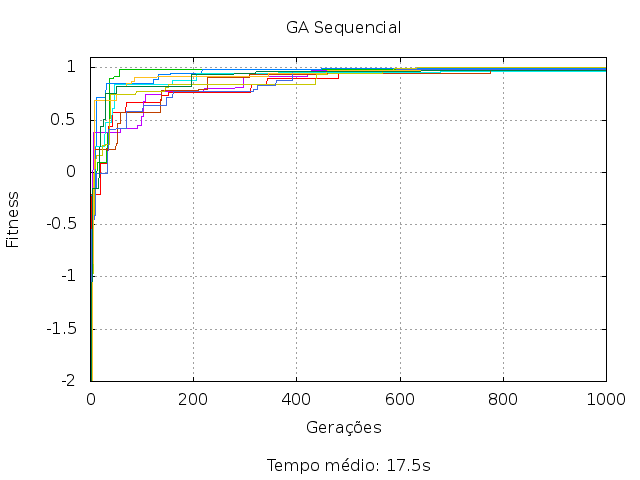
\includegraphics[width=0.8\textwidth]{seq_f1.png}
  \caption{GA Sequencial - Função \emph{Sphere}}
\end{figure}

\begin{figure}[hp]
  \centering
  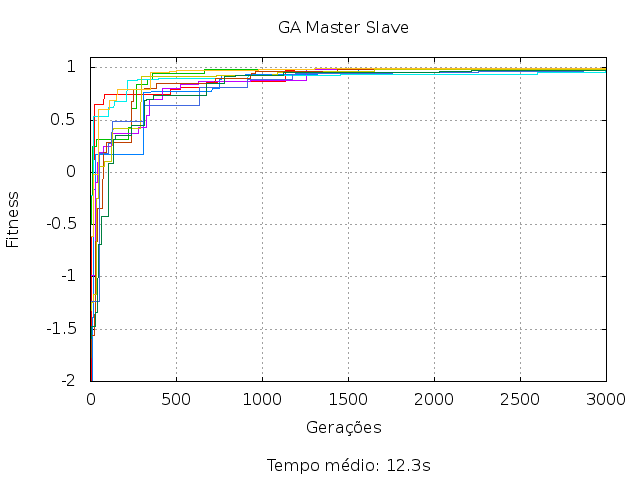
\includegraphics[width=0.8\textwidth]{ms_f1.png}
  \caption{GA \emph{Master-slave} - Função \emph{Sphere}}
\end{figure}

\begin{figure}[hp]
  \centering
  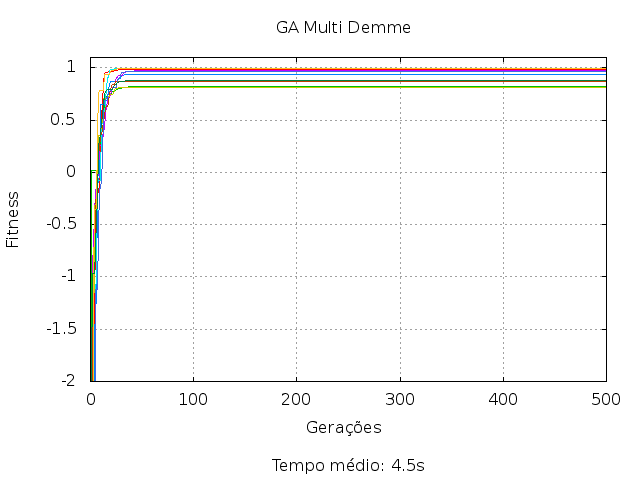
\includegraphics[width=0.8\textwidth]{md_f1.png}
  \caption{GA \emph{Multi-demme} - Função \emph{Sphere}}
\end{figure}

\begin{figure}[hp]
  \centering
  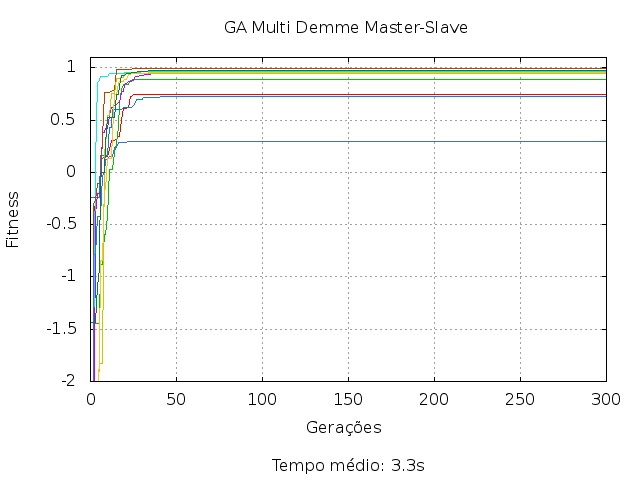
\includegraphics[width=0.8\textwidth]{msmd_f1.png}
  \caption{GA \emph{Multi-demme Master-Slave} - Função \emph{Sphere}}
\end{figure}


\begin{figure}[hp]
  \centering
  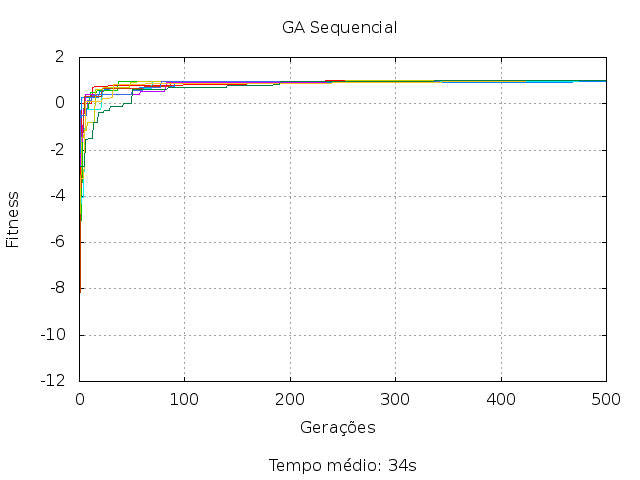
\includegraphics[width=0.8\textwidth]{seq_f2.png}
  \caption{GA Sequencial - Função \emph{Rotated Hyper-ellipsoid}}
\end{figure}

\begin{figure}[hp]
  \centering
  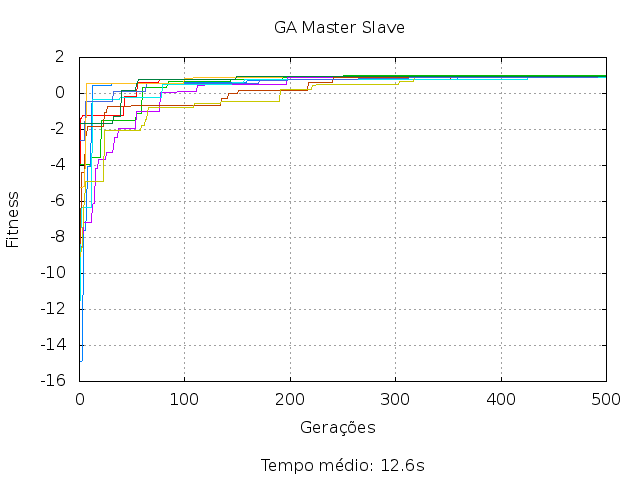
\includegraphics[width=0.8\textwidth]{ms_f2.png}
  \caption{GA \emph{Master-slave} - Função \emph{Rotated Hyper-ellipsoid}}
\end{figure}

\begin{figure}[hp]
  \centering
  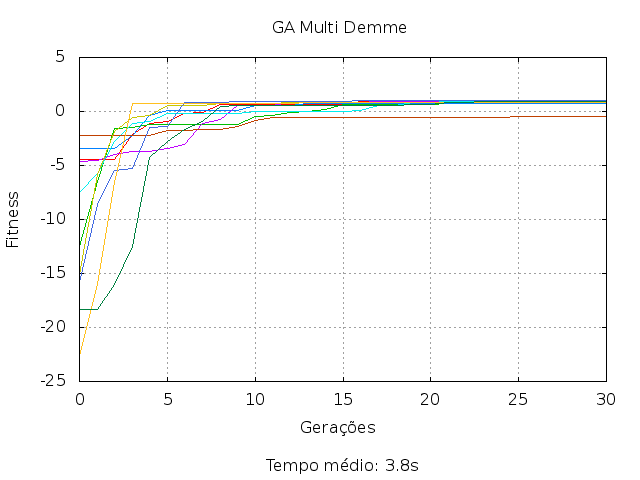
\includegraphics[width=0.8\textwidth]{md_f2.png}
  \caption{GA \emph{Multi-demme} - Função \emph{Rotated Hyper-ellipsoid}}
\end{figure}

\begin{figure}[hp]
  \centering
  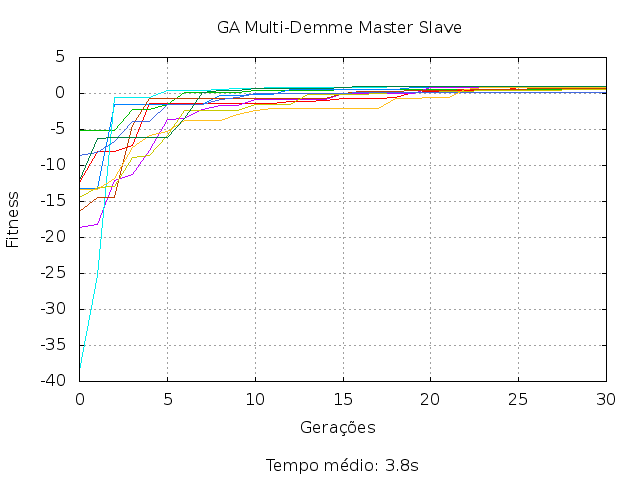
\includegraphics[width=0.8\textwidth]{mdms_f2.png}
  \caption{GA \emph{Multi-demme Master-Slave} - Função \emph{Rotated Hyper-ellipsoid}}
\end{figure}

\begin{figure}[hp]
  \centering
  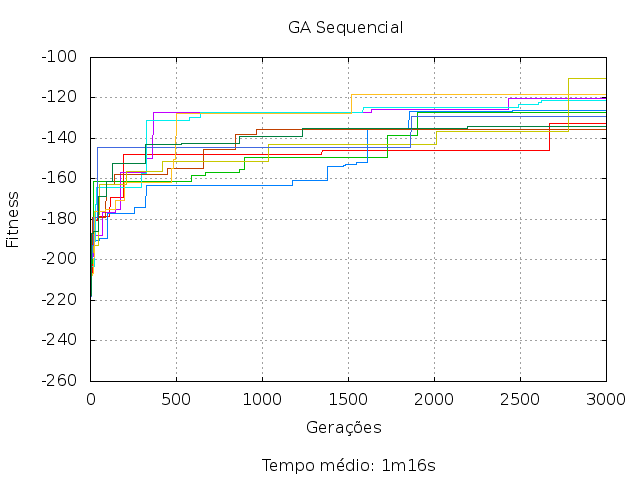
\includegraphics[width=0.8\textwidth]{seq_f3.png}
  \caption{GA Sequencial - Função \emph{Rastrigin}}
\end{figure}

\begin{figure}[hp]
  \centering
  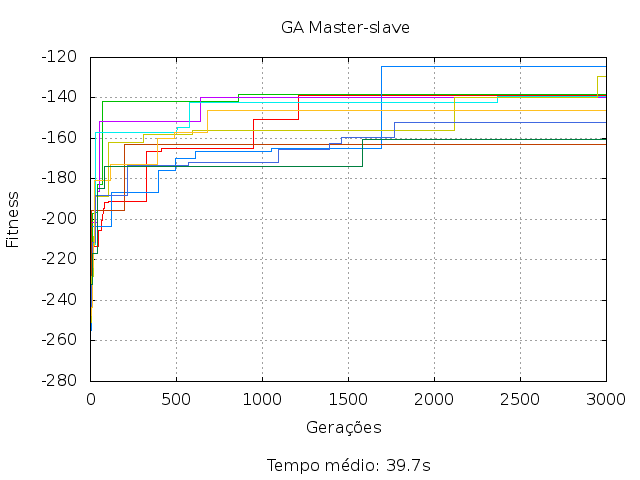
\includegraphics[width=0.8\textwidth]{ms_f3.png}
  \caption{GA \emph{Master-slave} - Função \emph{Rastrigin}}
\end{figure}

\begin{figure}[hp]
  \centering
  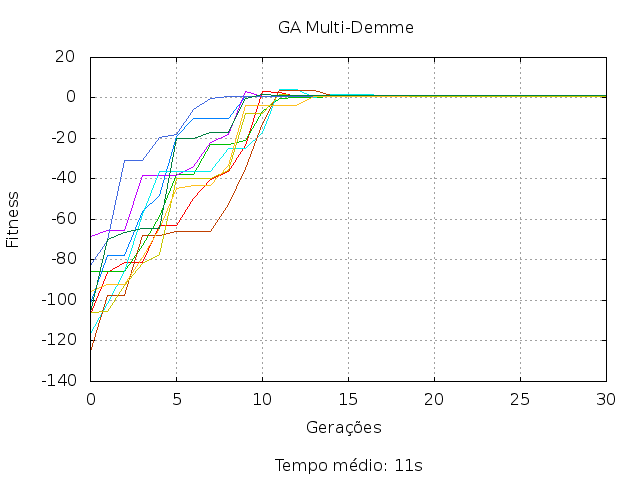
\includegraphics[width=0.8\textwidth]{md_f3.png}
  \caption{GA \emph{Multi-demme} - Função \emph{Rastrigin}}
\end{figure}

\begin{figure}[ht!p]
  \centering
  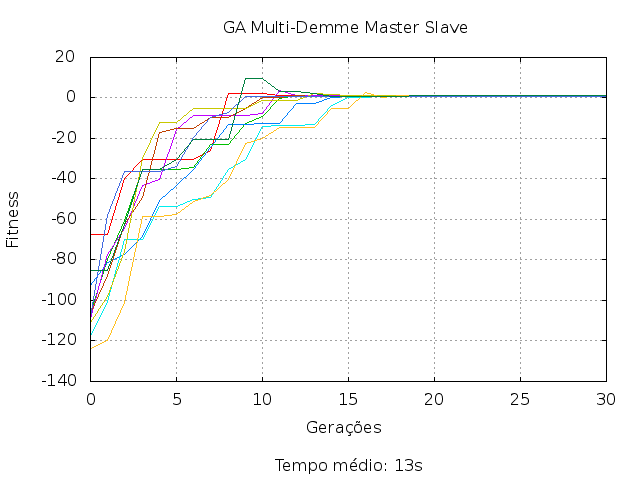
\includegraphics[width=0.8\textwidth]{mdms_f3.png}
  \caption{GA \emph{Multi-demme Master-Slave} - Função \emph{Rastrigin}}
\end{figure}


% subsection resultados (end)

% subsubsection pg_h (end)

% subsection algoritmos (end)

% subsubsection modelagem (end)
\newpage

\section{Conclusão} % (fold)
\label{sec:conclusao}
% section conclus_o (end)



% Esboço: Comparação entre ag tradicional, ag paralelo com multiplas populações, ag paralelo master slave e ag hibrido das duas anteriores.

% Problema: funções de de jong.

% Modelagem: Vetor de números reais. Cruzamento convencional. Mutação: pequena soma/subtração de número entre 0.01 e 0.05. Seleção torneio.

% Análise: tabelas: tempo gasto, resultado médio em 10 execuções para cada um dos ag's, ótimo conhecido. Gráfico: fitness x geração, testes: kruskal-wallis e/ou analise de covariancia (ancova).

% section experimentos (end)
\bibliographystyle{sbc}
\bibliography{rel}

\end{document}
